%!TEX root = ../thesis.tex
% ******************************* Thesis Appendix A ****************************

\chapter{}
\section{N-1 plots for cut-scan results}\label{app:n-1_plots_cut_opt}

\ifpdf
\graphicspath{{chapter-optimisation/Figs/Raster/}{chapter-electroweak/Figs/PDF/}{chapter-optimisation/Figs/}}
\else
\graphicspath{{chapter-optimisation/Figs/Vector/}{chapter-electroweak/Figs/}}
\fi

\begin{figure}
	\centering
	\begin{subfigure}[b]{0.5\linewidth}
		\centering\includegraphics[width=\textwidth]{N-1/n1_250_60_best_cut/met}
		\caption{\label{fig:result_250_60_met}}
	\end{subfigure}%
	\begin{subfigure}[b]{0.5\linewidth}
		\centering\includegraphics[width=\textwidth]{N-1/n1_250_60_best_cut/metsig}
		\caption{\label{fig:result_250_60_metsig}}
	\end{subfigure}
	\begin{subfigure}[b]{0.5\linewidth}
		\centering\includegraphics[width=\textwidth]{N-1/n1_250_60_best_cut/meff}
		\caption{\label{fig:result_250_60_meff}}
	\end{subfigure}%
	\begin{subfigure}[b]{0.5\linewidth}
		\centering\includegraphics[width=\textwidth]{N-1/n1_250_60_best_cut/mt}
		\caption{\label{fig:result_250_60_mt}}
	\end{subfigure}
	\begin{subfigure}[b]{0.5\linewidth}
		\centering\includegraphics[width=\textwidth]{N-1/n1_250_60_best_cut/nJet30}
		\caption{\label{fig:result_250_60_njet}}
	\end{subfigure}%
	\begin{subfigure}[b]{0.5\linewidth}
		\centering\includegraphics[width=\textwidth]{N-1/n1_250_60_best_cut/nBJet}
		\caption{\label{fig:result_250_60_nbjet}}
	\end{subfigure}
	\caption[N-1 plots for the chosen cut combination for the (250,60) signal point, 1/2]{First set of N-1 plots for the chosen cut combination for the \textbf{(250, 60)} signal point. These plots form the basis for a manual optimisation step that removes some of the unnecessary cuts or tweaks suboptimal cuts to better values.}
	\label{fig:results_250_60_n-1_1}
\end{figure}

\begin{figure}
	\centering
	\begin{subfigure}[b]{0.5\linewidth}
		\centering\includegraphics[width=\textwidth]{N-1/n1_250_60_best_cut/jet1Pt}
		\caption{\label{fig:result_250_60_jet1Pt}}
	\end{subfigure}%                              
	\begin{subfigure}[b]{0.5\linewidth}
		\centering\includegraphics[width=\textwidth]{N-1/n1_250_60_best_cut/jet2Pt}
		\caption{\label{fig:result_250_60_jet2Pt}}
	\end{subfigure}	
	\begin{subfigure}[b]{0.5\linewidth}
		\centering\includegraphics[width=\textwidth]{N-1/n1_250_60_best_cut/lep1Pt}
		\caption{\label{fig:result_250_60_lep1Pt}}
	\end{subfigure}%
	\begin{subfigure}[b]{0.5\linewidth}
		\centering\includegraphics[width=\textwidth]{N-1/n1_250_60_best_cut/dphimetlep}
		\caption{\label{fig:result_250_60_dphimetlep}}
	\end{subfigure}
	\begin{subfigure}[b]{0.5\linewidth}
		\centering\includegraphics[width=\textwidth]{N-1/n1_250_60_best_cut/mjj_upper_alone}
		\caption{\label{fig:result_250_60_mjj_upper}}
	\end{subfigure}%
	\begin{subfigure}[b]{0.5\linewidth}
		\centering\includegraphics[width=\textwidth]{N-1/n1_250_60_best_cut/dRJet}
		\caption{\label{fig:result_250_60_dRJet}}
	\end{subfigure}
	\caption[N-1 plots for the chosen cut combination for the (250,60) signal point, 2/2]{Second set of N-1 plots for the chosen cut combination for the \textbf{(250, 60)} signal point. These plots form the basis for a manual optimisation step that removes some of the unnecessary cuts or tweaks suboptimal cuts to better values. In \figname~\subref{fig:result_250_60_mjj_upper}, for illustration purposes, the lower requirement is not applied while the upper cut is scanned.}
	\label{fig:results_250_60_n-1}
\end{figure}

\begin{figure}
	\centering
	\begin{subfigure}[b]{0.5\linewidth}
		\centering\includegraphics[width=\textwidth]{N-1/n1_300_0_best_cut/met}
		\caption{\label{fig:result_300_0_met}}
	\end{subfigure}%
	\begin{subfigure}[b]{0.5\linewidth}
		\centering\includegraphics[width=\textwidth]{N-1/n1_300_0_best_cut/metsig}
		\caption{\label{fig:result_300_0_metsig}}
	\end{subfigure}
	\begin{subfigure}[b]{0.5\linewidth}
		\centering\includegraphics[width=\textwidth]{N-1/n1_300_0_best_cut/meff}
		\caption{\label{fig:result_300_0_meff}}
	\end{subfigure}%
	\begin{subfigure}[b]{0.5\linewidth}
		\centering\includegraphics[width=\textwidth]{N-1/n1_300_0_best_cut/mt}
		\caption{\label{fig:result_300_0_mt}}
	\end{subfigure}
	\begin{subfigure}[b]{0.5\linewidth}
		\centering\includegraphics[width=\textwidth]{N-1/n1_300_0_best_cut/nJet30}
		\caption{\label{fig:result_300_0_njet}}
	\end{subfigure}%
	\begin{subfigure}[b]{0.5\linewidth}
		\centering\includegraphics[width=\textwidth]{N-1/n1_300_0_best_cut/nBJet}
		\caption{\label{fig:result_300_0_nbjet}}
	\end{subfigure}
	\caption[N-1 plots for the chosen cut combination for the (300,0) signal point, 1/2]{First set of N-1 plots for the chosen cut combination for the \textbf{(300, 0)} signal point. These plots form the basis for a manual optimisation step that removes some of the unnecessary cuts or tweaks suboptimal cuts to better values.}
	\label{fig:results_300_0_n-1_1}
\end{figure}

\begin{figure}
	\centering
	\begin{subfigure}[b]{0.5\linewidth}
		\centering\includegraphics[width=\textwidth]{N-1/n1_300_0_best_cut/jet1Pt}
		\caption{\label{fig:result_300_0_jet1Pt}}
	\end{subfigure}%                              
	\begin{subfigure}[b]{0.5\linewidth}
		\centering\includegraphics[width=\textwidth]{N-1/n1_300_0_best_cut/jet2Pt}
		\caption{\label{fig:result_300_0_jet2Pt}}
	\end{subfigure}	
	\begin{subfigure}[b]{0.5\linewidth}
		\centering\includegraphics[width=\textwidth]{N-1/n1_300_0_best_cut/lep1Pt}
		\caption{\label{fig:result_300_0_lep1Pt}}
	\end{subfigure}%
	\begin{subfigure}[b]{0.5\linewidth}
		\centering\includegraphics[width=\textwidth]{N-1/n1_300_0_best_cut/dphimetlep}
		\caption{\label{fig:result_300_0_dphimetlep}}
	\end{subfigure}
	\begin{subfigure}[b]{0.5\linewidth}
		\centering\includegraphics[width=\textwidth]{N-1/n1_300_0_best_cut/mjj_upper_alone}
		\caption{\label{fig:result_300_0_mjj_upper}}
	\end{subfigure}%
	\begin{subfigure}[b]{0.5\linewidth}
		\centering\includegraphics[width=\textwidth]{N-1/n1_300_0_best_cut/dRJet}
		\caption{\label{fig:result_300_0_dRJet}}
	\end{subfigure}
	\caption[N-1 plots for the chosen cut combination for the (300,0) signal point, 2/2]{Second set of N-1 plots for the chosen cut combination for the \textbf{(300, 0)} signal point. These plots form the basis for a manual optimisation step that removes some of the unnecessary cuts or tweaks suboptimal cuts to better values. In \figname~\subref{fig:result_300_0_mjj_upper}, for illustration purposes, the lower requirement is not applied while the upper cut is scanned.}
	\label{fig:results_300_0_n-1}
\end{figure}

\begin{figure}
	\centering
	\begin{subfigure}[b]{0.5\linewidth}
		\centering\includegraphics[width=\textwidth]{N-1/n1_400_0_best_cut/met}
		\caption{\label{fig:result_400_0_met}}
	\end{subfigure}%
	\begin{subfigure}[b]{0.5\linewidth}
		\centering\includegraphics[width=\textwidth]{N-1/n1_400_0_best_cut/metsig}
		\caption{\label{fig:result_400_0_metsig}}
	\end{subfigure}
	\begin{subfigure}[b]{0.5\linewidth}
		\centering\includegraphics[width=\textwidth]{N-1/n1_400_0_best_cut/meff}
		\caption{\label{fig:result_400_0_meff}}
	\end{subfigure}%
	\begin{subfigure}[b]{0.5\linewidth}
		\centering\includegraphics[width=\textwidth]{N-1/n1_400_0_best_cut/mt}
		\caption{\label{fig:result_400_0_mt}}
	\end{subfigure}
	\begin{subfigure}[b]{0.5\linewidth}
		\centering\includegraphics[width=\textwidth]{N-1/n1_400_0_best_cut/nJet30}
		\caption{\label{fig:result_400_0_njet}}
	\end{subfigure}%
	\begin{subfigure}[b]{0.5\linewidth}
		\centering\includegraphics[width=\textwidth]{N-1/n1_400_0_best_cut/nBJet}
		\caption{\label{fig:result_400_0_nbjet}}
	\end{subfigure}
	\caption[N-1 plots for the chosen cut combination for the (400,0) signal point, 1/2]{First set of N-1 plots for the chosen cut combination for the \textbf{(400, 0)} signal point. These plots form the basis for a manual optimisation step that removes some of the unnecessary cuts or tweaks suboptimal cuts to better values.}
	\label{fig:results_400_0_n-1_1}
\end{figure}

\begin{figure}
	\centering
	\begin{subfigure}[b]{0.5\linewidth}
		\centering\includegraphics[width=\textwidth]{N-1/n1_400_0_best_cut/jet1Pt}
		\caption{\label{fig:result_400_0_jet1Pt}}
	\end{subfigure}%                              
	\begin{subfigure}[b]{0.5\linewidth}
		\centering\includegraphics[width=\textwidth]{N-1/n1_400_0_best_cut/jet2Pt}
		\caption{\label{fig:result_400_0_jet2Pt}}
	\end{subfigure}	
	\begin{subfigure}[b]{0.5\linewidth}
		\centering\includegraphics[width=\textwidth]{N-1/n1_400_0_best_cut/lep1Pt}
		\caption{\label{fig:result_400_0_lep1Pt}}
	\end{subfigure}%
	\begin{subfigure}[b]{0.5\linewidth}
		\centering\includegraphics[width=\textwidth]{N-1/n1_400_0_best_cut/dphimetlep}
		\caption{\label{fig:result_400_0_dphimetlep}}
	\end{subfigure}
	\begin{subfigure}[b]{0.5\linewidth}
		\centering\includegraphics[width=\textwidth]{N-1/n1_400_0_best_cut/mjj_upper_alone}
		\caption{\label{fig:result_400_0_mjj_upper}}
	\end{subfigure}%
	\begin{subfigure}[b]{0.5\linewidth}
		\centering\includegraphics[width=\textwidth]{N-1/n1_400_0_best_cut/dRJet}
		\caption{\label{fig:result_400_0_dRJet}}
	\end{subfigure}
	\caption[N-1 plots for the chosen cut combination for the (400,0) signal point, 2/2]{Second set of N-1 plots for the chosen cut combination for the \textbf{(400, 0)} signal point. These plots form the basis for a manual optimisation step that removes some of the unnecessary cuts or tweaks suboptimal cuts to better values. In \figname~\subref{fig:result_400_0_mjj_upper}, for illustration purposes, the lower requirement is not applied while the upper cut is scanned.}
	\label{fig:results_400_0_n-1}
\end{figure}

\begin{figure}
	\centering
	\begin{subfigure}[b]{0.5\linewidth}
		\centering\includegraphics[width=\textwidth]{N-1/n1_500_0_best_cut/met}
		\caption{\label{fig:result_500_0_met}}
	\end{subfigure}%
	\begin{subfigure}[b]{0.5\linewidth}
		\centering\includegraphics[width=\textwidth]{N-1/n1_500_0_best_cut/metsig}
		\caption{\label{fig:result_500_0_metsig}}
	\end{subfigure}
	\begin{subfigure}[b]{0.5\linewidth}
		\centering\includegraphics[width=\textwidth]{N-1/n1_500_0_best_cut/meff}
		\caption{\label{fig:result_500_0_meff}}
	\end{subfigure}%
	\begin{subfigure}[b]{0.5\linewidth}
		\centering\includegraphics[width=\textwidth]{N-1/n1_500_0_best_cut/mt}
		\caption{\label{fig:result_500_0_mt}}
	\end{subfigure}
	\begin{subfigure}[b]{0.5\linewidth}
		\centering\includegraphics[width=\textwidth]{N-1/n1_500_0_best_cut/nJet30}
		\caption{\label{fig:result_500_0_njet}}
	\end{subfigure}%
	\begin{subfigure}[b]{0.5\linewidth}
		\centering\includegraphics[width=\textwidth]{N-1/n1_500_0_best_cut/nBJet}
		\caption{\label{fig:result_500_0_nbjet}}
	\end{subfigure}
	\caption[N-1 plots for the chosen cut combination for the (500,0) signal point, 1/2]{First set of N-1 plots for the chosen cut combination for the \textbf{(500, 0)} signal point. These plots form the basis for a manual optimisation step that removes some of the unnecessary cuts or tweaks suboptimal cuts to better values.}
	\label{fig:results_500_0_n-1_1}
\end{figure}

\begin{figure}
	\centering
	\begin{subfigure}[b]{0.5\linewidth}
		\centering\includegraphics[width=\textwidth]{N-1/n1_500_0_best_cut/jet1Pt}
		\caption{\label{fig:result_500_0_jet1Pt}}
	\end{subfigure}%                              
	\begin{subfigure}[b]{0.5\linewidth}
		\centering\includegraphics[width=\textwidth]{N-1/n1_500_0_best_cut/jet2Pt}
		\caption{\label{fig:result_500_0_jet2Pt}}
	\end{subfigure}	
	\begin{subfigure}[b]{0.5\linewidth}
		\centering\includegraphics[width=\textwidth]{N-1/n1_500_0_best_cut/lep1Pt}
		\caption{\label{fig:result_500_0_lep1Pt}}
	\end{subfigure}%
	\begin{subfigure}[b]{0.5\linewidth}
		\centering\includegraphics[width=\textwidth]{N-1/n1_500_0_best_cut/dphimetlep}
		\caption{\label{fig:result_500_0_dphimetlep}}
	\end{subfigure}
	\begin{subfigure}[b]{0.5\linewidth}
		\centering\includegraphics[width=\textwidth]{N-1/n1_500_0_best_cut/mjj_upper_alone}
		\caption{\label{fig:result_500_0_mjj_upper}}
	\end{subfigure}%
	\begin{subfigure}[b]{0.5\linewidth}
		\centering\includegraphics[width=\textwidth]{N-1/n1_500_0_best_cut/dRJet}
		\caption{\label{fig:result_500_0_dRJet}}
	\end{subfigure}
	\caption[N-1 plots for the chosen cut combination for the (500,0) signal point, 2/2]{Second set of N-1 plots for the chosen cut combination for the \textbf{(500, 0)} signal point. These plots form the basis for a manual optimisation step that removes some of the unnecessary cuts or tweaks suboptimal cuts to better values. In \figname~\subref{fig:result_500_0_mjj_upper}, for illustration purposes, the lower requirement is not applied while the upper cut is scanned.}
	\label{fig:results_500_0_n-1}
\end{figure}